\documentclass[urlcolor=blue,dvipsnames]{beamer}

\usepackage[utf8]{inputenc}
\usepackage{fancybox,fancyvrb}
\usepackage{environ,xspace}
\usepackage{tikz}
\hypersetup{colorlinks,linkcolor=,urlcolor=cyan}

\beamertemplatenavigationsymbolsempty
\setbeamertemplate{footline}[frame number]
\usetheme{Pittsburgh}

\newcommand\enumnum[1]{{\renewcommand{\insertenumlabel}{#1}%
      \usebeamertemplate{enumerate item} \,}}

\newcommand{\grad}{\nabla}
\newcommand{\ih}{\boldsymbol{\hat{\textbf{\i}}}}
\newcommand{\jh}{\boldsymbol{\hat{\textbf{\j}}}}
\newcommand{\vF}{\boldsymbol{\vec{\textbf{F}}}}
\newcommand{\Matlab}{\textsc{Matlab}\xspace}
\newcommand{\Octave}{\textsc{Octave}\xspace}


\title{6.1 Power series solutions of DEs \\ (and review)}

\subtitle{a lesson for MATH F302 Differential Equations}

\author{Ed Bueler, Dept.~of Mathematics and Statistics, UAF}

\date{\tiny \today}


\begin{document}
\setbeamertemplate{itemize item}{$\bullet$}
\setbeamertemplate{itemize subitem}{$\circ$}


\begin{frame}
\titlepage

\centerline{\tiny for textbook: \, D. Zill, \emph{A First Course in Differential Equations with Modeling Applications}, 11th ed.}
%\color{green!40!blue}
\end{frame}


\begin{frame}{we already use power series}

\begin{itemize}
\item the exponential function is \emph{defined} by an infinite series:
    $$e^x = 1 + x + \frac{x^2}{2} + \frac{x^3}{3!} + \dots$$
    \begin{itemize}
    \item there are other ways to define the exponential but the above is the default definition; see \href{https://en.wikipedia.org/wiki/Characterizations_of_the_exponential_function}{``characterizations of the exponential function''} at wikipedia
    \end{itemize}
\item a \emph{power series} is an infinite sum of coefficients times powers of $x$; the above is a power series
\item \emph{exercise.} from the above series for $y(x)=e^x$, show
    $$y'=y \,\, \text{ and } \,\, y(0)=1$$
\end{itemize}

\vspace{30mm}
\end{frame}


\begin{frame}{try a series with unknown coefficients}

\noindent \emph{exercise.}  find the coefficients in the power series
    $$y(x) = c_0 + c_1 x + c_2 x^2 + c_3 x^3 + c_4 x^4 + \dots$$
so that $y(x)$ solves the IVP: \quad $y'+3y=0, \, y(0) = 7$

\vspace{60mm}
\end{frame}


\begin{frame}{exercise \#37 in \S 6.1}

\noindent \emph{exercise.}  find the general solution by using a series:
    $$y'=xy$$

\vspace{70mm}
\end{frame}


\begin{frame}{review of series}

\begin{itemize}
\item reviewing series includes recalling at least these three things from calculus II:
    \begin{enumerate}
    \item some familiar series
        \begin{itemize}
        \item including little tricks to get to a few other familiar series
        \end{itemize}
    \item how summation notation works
    \item what are the \emph{radius of convergence} and the \emph{interval of convergence}, and how to find them
    \end{enumerate}

\bigskip
\item to do \emph{your} review, start by \alert{reading the text in section 6.1}!!
\end{itemize}
\end{frame}


\begin{frame}{X}

\begin{itemize}
\item X
\end{itemize}
\end{frame}

\begin{frame}{X}

\begin{itemize}
\item X
\end{itemize}
\end{frame}




\begin{frame}{familiar series}

\begin{itemize}
\item X
\end{itemize}

\hfill 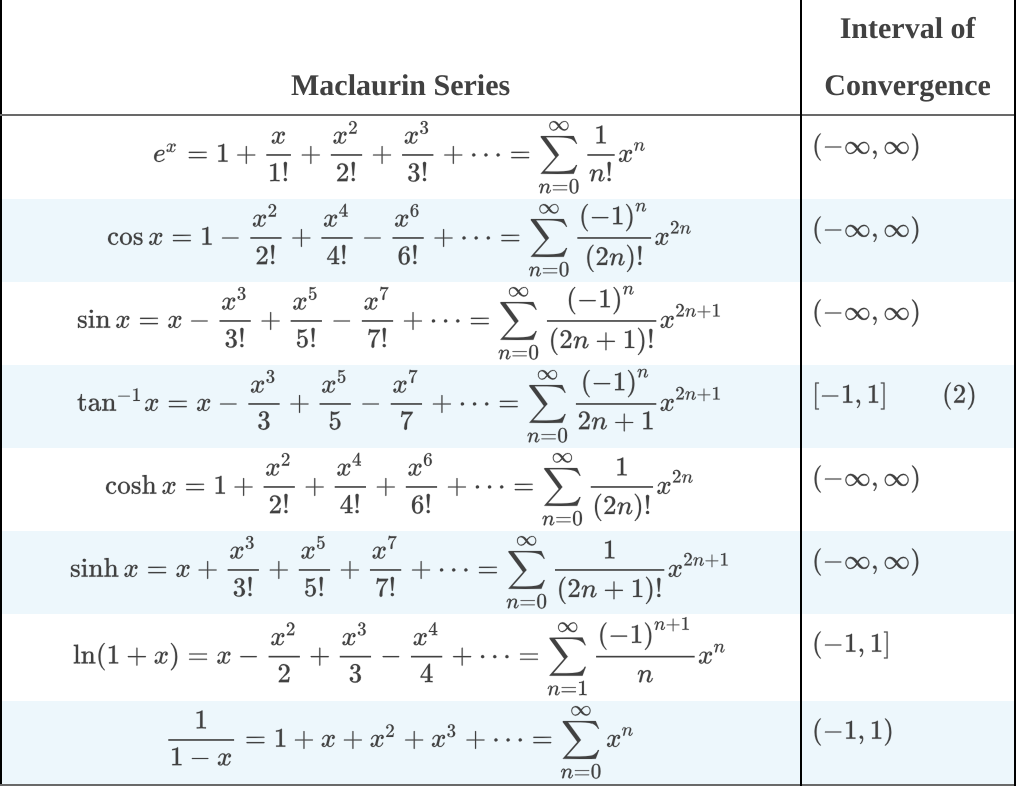
\includegraphics[width=0.6\textwidth]{figs/familiarseries}
\end{frame}


\begin{frame}{exercise \#14 in \S 6.1}

\noindent \emph{exercise.}  Use a familiar series to find the Maclaurin series of the given function.  Write your answer in summation notation.

$$\frac{x}{1+x^2} \hspace{60mm}$$

\vspace{60mm}
\end{frame}


\begin{frame}{exercise \#31 in \S 6.1}

\noindent \emph{exercise.}  Verify by direct substitution that the given power series is a soltuion of the DE.  (Use manipulations of summation notation to do your calculation.)  What is the radius of convergence of the series solution?

$$y=\sum_{n=0}^\infty \frac{(-1)^n}{n!} x^{2n}, \qquad\quad y'+2xy=0$$

\vspace{60mm}
\end{frame}


\begin{frame}{exercise \#31, cont.}

\end{frame}


\begin{frame}{convergence and divergence of power series}

\begin{itemize}
\item X
\end{itemize}

\hfill 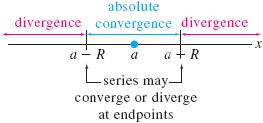
\includegraphics[width=0.45\textwidth]{figs/convergediverge}
\end{frame}


\begin{frame}{exercise \#5 in \S 6.1}

\noindent \emph{exercise.}  Find the interval and radius of convergence for the given power series.
    $$\sum_{k=1}^\infty \frac{(-1)^k}{10^k} (x-5)^k$$

\vspace{60mm}
\end{frame}


\begin{frame}{exercise \#33 in \S 6.1}

\noindent \emph{exercise.}  

\vspace{60mm}
\end{frame}


\begin{frame}{X}

\begin{itemize}
\item X
\end{itemize}
\end{frame}


\begin{frame}{expectations}

\begin{itemize}
\item just watching this video is \emph{not} enough!
     \begin{itemize}
     \item see ``found online'' videos at

     \centerline{\href{https://bueler.github.io/math302/week9.html}{\tt \color{cyan} bueler.github.io/math302/week9.html}}
     \item \emph{read} section 6.1 and 6.2 in the textbook
     \item \emph{do} the WebAssign exercises for section 6.1
     \end{itemize}
\end{itemize}
\end{frame}

\end{document}

